\documentclass[times, utf8, diplomski, numeric, english]{fer}

\usepackage{booktabs}
\usepackage{amsmath}
\usepackage{nccmath}
%\usepackage{hyperref}
\usepackage[section]{placeins}

\usepackage{footnote}
\usepackage{graphicx}
\usepackage{float}
\usepackage{mathtools}
\usepackage{makecell}

\renewcommand\theadalign{cb}
\renewcommand\theadfont{\bfseries}
\renewcommand\theadgape{\Gape[4pt]}
\renewcommand\cellgape{\Gape[4pt]}

\DeclarePairedDelimiter\ceil{\lceil}{\rceil}
\DeclarePairedDelimiter\floor{\lfloor}{\rfloor}

\DeclareMathOperator*{\argmin}{\arg\!\min}
\DeclareMathOperator*{\argmax}{\arg\!\max}
\begin{document}


\thesisnumber{1417}
\title{Deep Learning Model for Base Calling of MinION Nanopore Reads}
\author{Marko Ratković}

\maketitle

% Ispis stranice s napomenom o umetanju izvornika rada. Uklonite naredbu \izvornik ako želite izbaciti tu stranicu.
\izvornik

% Dodavanje zahvale ili prazne stranice. Ako ne želite dodati zahvalu, naredbu ostavite radi prazne stranice.
\zahvala{Thanks ...}

\tableofcontents
\listoffigures
\listoftables

%%%%%%%%%%%%%%%%%%%%%%%%%%%%%%%%%%%%%%%%%%%%%%%%%%%%%%%%%%%%%%%%%%%%%%%%%%%%%%%%%%%%%%%
%% CHAPTER
\chapter{Introduction}

In recent years,  deep learning methods significantly improved the state-of-the-art in multiple domains such as computer vision, speech recognition, and natural language processing\cite{LeCun:1998:CNI:303568.303704}\cite{NIPS2012_4824}. 
In this thesis, we present application of deep learning in the fields of Biology and Bioinformatics for analysis of DNA sequencing data. 

DNA is a molecule that makes up the genetic material of a cell and it is responsible for carrying the information needed for survival, growth, and reproduction of an organism. 
DNA is a long polymer of simple blocks called nucleotides connected together to form two spiraling strands to a structure called a double helix.  Possible nucleotide bases of a DNA strand are adenine, cytosine, guanine, thymine usually represented with letters A, C, G, and T,   The order of these bases is what defines genetic code.

DNA sequencing is the process of determining this sequence of nucleotides. Originally sequencing was an expensive process but during the last couple of decades, the price of sequencing has drastically decreased.  A significant breakthrough occurred in May 2015 with the release of MinION sequencer by Oxford Nanopore making DNA sequencing inexpensive and more available, even for small research teams. 

Base calling is a process assigning sequence of nucleotides (letters) to the raw data generated by the sequencing device or sequencer. Simply put, it is a process of decoding the output from the sequencer.


\section{Objectives}
The goal of this thesis is to show that the accuracy of base calling is dependent on the underlying software and can be improved using machine learning methods. A novel approach for base calling of raw data using convolutional neural networks is introduced.

\section{Organization}
\indent Chapter 2 gives more detailed explanation of the problem, background on nanopore sequencing and overview of state-of-the-art basecallers.

Chapter 3 describes in detail deep learning concepts discussed in later chapters.

Chapter 4 goes into implementation details, training of the deep learning model and explains the methodology used to evaluate obtained results. 

Chapter 5 consists of the results of testing performed on different datasets as well as comparison with state-of-the-art basecallers.

In the end, Chapter 6 gives a brief conclusion and possible future work and improvements of the developed basecaller.

%%%%%%%%%%%%%%%%%%%%%%%%%%%%%%%%%%%%%%%%%%%%%%%%%%%%%%%%%%%%%%%%%%%%%%%%%%%%%%%%%%%%%%%
%% CHAPTER
\chapter{Background}

\section{Sequencing}

All sequencing technologies to date have constraints on the length of the strand they can process which are much smaller than the genome for a majority of organisms, making sequencing the entire genome of an organism is a difficult problem. To resolve this problem whole genome shotgun sequencing approach is used, in which multiple copies of the genome are broken up randomly into numerous small fragments that can be processed by the sequencer. Sequenced fragments are called reads.

Genome assembly is the process of reconstructing the original genome from reads and usually starts with finding overlaps between reads.
The quality of reconstruction heavily depends on the length and accuracy of the reads produced by the sequencer.

Figure \ref{fg:sequencing} depicts process of sequencing.

\begin{figure}[!ht]
	\begin{center}
		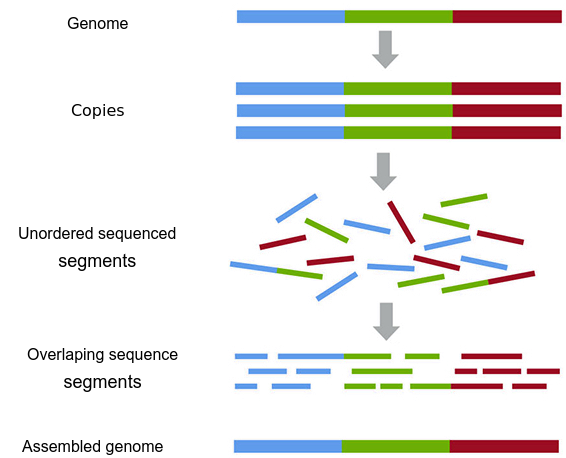
\includegraphics[width=0.6\textwidth]{./imgs/sequencing.png}
		\caption{Depiction of the sequencing process}
		\label{fg:sequencing}
	\end{center}
\end{figure}


Development of sequencing started with work of Frederick Sanger\cite{mile}\cite{Pettersson2009}. In 1977, he developed the first sequencing method which allowed 
read lengths up to 1000 bases with very high accuracy (99.9\%) at a cost of 1\$ per 1000 bases[mile\_skripta].
Second generation sequencing (IAN Torrent and Illumina devices) reduced the price of sequencing while maintaining high accuracy. Mayor disadvantage of these devices is read length of only a few hundred base pairs. Short reads make resolving repetitive regions practically impossible.

The need for technologies that would produce longer reads led to the development of so-called third generation sequencing technologies.
PacBio developed sequencing method that allowed read lengths up to several thousand bases but at a cost of accuracy. Error Rates of PacBio devices are ~10-15\%. 

Cost makes the main obstacle stopping widespread genome sequencing. The release of, previously mentioned, MinION sequencer made sequencing drastically less expensive and even portable.


\section{Oxford Nanopore MinION}

The MinION device by Oxford Nanopore Technologies is the first portable DNA sequencing device. It’s small weight, low cost, and long read length combined with decent accuracy yield promising results in various applications including full human genome assembly\cite{human_seq} what could potentially lead to personalized genomic medicine.

\subsection{Technology}
As its name says, pores of nanoscale are used to sequence DNA. An electrical potential is applied over a membrane in which a  pore is inserted. 
As the DNA passes through the pore, the sensor detects changes in ionic current caused by differences nucleotides present in the pore. Figure \ref{fg:nanopore} shows the change of ionic current as DNA strain is pulled through a nanopore.

\begin{figure}[!ht]
	\begin{center}
		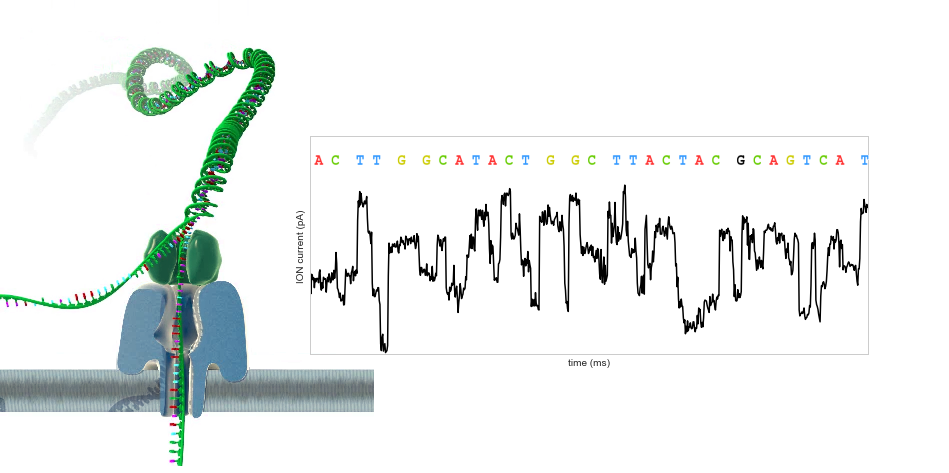
\includegraphics[width=0.7\textwidth]{./imgs/nanopore.png}
		
		\caption[DNA strain being pulled through a nanopore]{DNA strain being pulled through a nanopore \protect\footnotemark}
		\label{fg:nanopore}
	\end{center}
\end{figure}
\footnotetext{Figure adapted from https://nanoporetech.com/how-it-works}

Official software called MinKNOW outputs sequencing data in FAST5 (a variant of the HDF5 standard) file format. It is a hierarchical file format with data arranged in a tree-structure of groups. Metadata are stored in group and dataset attributes. The same file format is during used different stages of analyses and groups, datasets and attributes are added incrementally. Figure \ref{fg:fast5} shows raw signal being present in the FAST5 file.
\begin{figure}[!ht]
	\begin{center}
		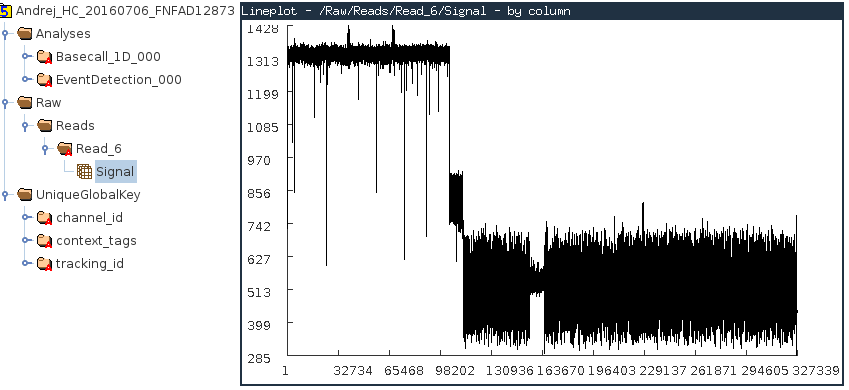
\includegraphics[width=0.6\textwidth]{./imgs/fast5.png}
		\caption[Structure of FAST5 file and raw signal plot show in \textit{HDFView}]{Structure of FAST5 file and raw signal line plot show in \textit{HDFView} \protect\footnotemark}
		\label{fg:fast5}
	\end{center}
\end{figure}
\footnotetext{https://support.hdfgroup.org/products/java/hdfview/}


Minion offers the possibility of sequencing one or both strands of DNA(1D or 2D reads). Combining information from both strands is results in reads of higher quality, 
MinION is able to produce long reads, usually tens of thousand base pairs (with reported reads lengths of 100 thousand \cite{loman1-100k} and even recently above 800 thousand base pairs \cite{loman2-800k}), but with high sequencing error than older generations of sequencing technologies.
Switch from older R7.3 to  R9 chemistry in 2016 increased accuracy of produced data. With this change, the accuracy of 1D data increased from 70\% to 85\% and the accuracy of 2D reads from 88\% to 94\%\cite{nanopore_video}.  This increase of accuracy makes 1D reads usable for analysis with benefits over 2D reads being faster sample preparation and faster sequencing. Developed tool will focus on base calling these kinds of reads.

  
\section{Existing basecallers}

\subsection{Official}
Oxford Nanopore has with the R9 version of the platform, introduced a variety of base calling options. Some of those are production ready and some experimental. The majority of information regarding differences, specifications and similar is only available through community nanoporetech \footnote. 
https://community.nanoporetech.com/


Metrichor is an Oxford Nanopore company, that offers cloud-based platform EPI2ME for analysis of nanopore data. 
Initially, base calling was only available by uploading data to the platform - that being the reason why this basecaller is often called Metrichor even though Metrichor is actually a name of the company.

Older version of Metrichor relied on hidden Markov models (HMM) to find the biological sequence corresponding to the signal. Preprocess included segmentation of the signal into smaller chunks called events defined by start location of the chunk, length, mean value and variance of the signal in the chunk. Metrichor than assumed that each event usually corresponds to a context of 5 bases being present in the pore and that the context is typically shifted by one base in each step. 
HMM states are modeled as a context present in the pore and transition correspond to change of bases in the pore. During the transition from one state to another, an event is emitted. Basecalling is performed using the Viterbi algorithm which determines the most likely sequence of states for the observed sequence of events. This approach showed poor results when calling long homopolymer stretches as the context in the pore remains the same\cite{homopolymers}.

With the release of R9 chemistry, this model was replaced by a more accurate recurrent neural network (RNN) implementation. Currently, Oxford Nanopore offers several RNN-based local basecaller versions under different names\cite{ont-basecallers}: Albacore, Nanonet and basecaller integrated into MinKNOW.  

\textbf{Albacore} is basecaller by Oxford Nanopore Technologies ready for production and actively supported.
It is available to the Nanopore Community served as a binary. The source code of Albacore was not provided and is only available through the ONT Developer Channel. 

\textbf{Nanonet}\footnote{\url{https://github.com/nanoporetech/nanonet/}} uses the same neural network that is used in Albacore but it is continually under development and does contain features such as error handling or logging needed for production use. It uses CURRENNT library for running neural networks.


\textbf{Scrappie}\footnote{\url{https://github.com/nanoporetech/scrappie}} is another basecaller by Oxford Nanopore Technologies. Similar to NanoNet, it is the platform for ongoing development. Scrappie is reported to be the first basecaller  that specifically address homopolymer basecalling. It became publicly available just recently in June, 2017.

\subsection{Third-party}

\textbf{Nanocall}\cite{David046086} was the first third-party open source basecaller for nanopore data. It uses HMM approach like the original R7 Metrichor. Nanocall does not support newer chemistries after R7.3.


\textbf{DeepNano}\cite{Boza2017}  was the first open-source basecaller based on neural networks that uses bidirectional recurrent neural networks. DeepNano was written in Python, using the Theano library. When released, originally only supported R7 chemistry, but support for R9 and R9.4 was added recently.



%%%%%%%%%%%%%%%%%%%%%%%%%%%%%%%%%%%%%%%%%%%%%%%%%%%%%%%%%%%%%%%%%%%%%%%%%%%%%%%%%%%%%%%
%% CHAPTER
\chapter{Methods}
The process of basecalling can be represented as the problem of machine translation where a sentence is translated from one language to another. For base calling, the sequence of events or current measurements is translated to the sequence of nucleotides (letters A, C, T, G).

This section explains some key concepts in deep learning needed to understand the final model. It gives general idea behind recurrent neural networks used in a majority of existing basecallers and possible difficulties that serve as motivation for the different approach, usage of convolutional neural networks. 

\section{Arhitecture}

\subsection{RNN}
\textit{Recurrent neural networks} can be viewed as a simple feed-forward network with the difference that the current output does not only depend on the current input but previous inputs as well. RNNs store that information in their hidden state and that state is updated in each step. The figure shows simple RNN and the same RNN unfolded in time.  Unrolling is a simple way of showing how network processes each input in the sequence and updates its hidden state (show in figure  \ref{fg:rnn}.( 
\begin{figure}[!ht]
	\begin{center}
		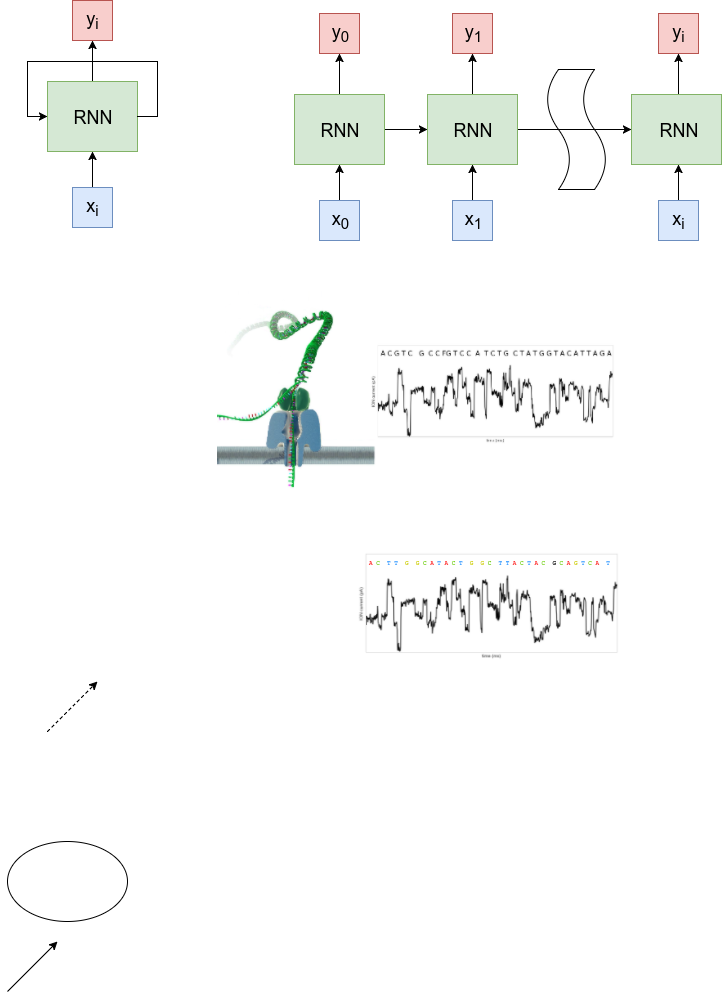
\includegraphics[width=0.8\textwidth]{./imgs/rnn.png}
		\caption{An unrolled recurrent neural network}
		\label{fg:rnn}
	\end{center}
\end{figure}

These networks are trained using a variant of backpropagation called backpropagation through time which is essentially the same as classical backpropagation on an unfolded network. The gradient is propagated through the entire recurrence relation and the gradient is multiplied in each step with the same factor, depending on a scale it can make gradient vanish (drop to 0) or exponentially grow each step and explode. Detailed explanation can be found \cite{rnn-blog}. These issues are called the vanishing and exploding gradient\cite{rnn-blog} and are generally resolved by a variant of RNN called \textit{LSTM}\cite{hochreiter1997long}. 

Bidirectional Recurrent Neural (BiRNN) networks are used when the current output not only depends on the previous elements in the sequence but also future elements. Idea is to combine two RNN (one in the positive direction, one in negative time direction) and have an output of the current state expressed as a function of hidden states of both RNNs and current input. This is the approach used in DeepNano\cite{Boza2017}. 


One of the major drawbacks of all recurrent networks is computation time. RNNs operate sequentially as the output for the second step depends on the first step and so on, which makes parallelization capabilities of RNNs quite limited. This especially goes for Bidirectional RNNs.

\subsection{CNN}

\textit{Convolutional Neural Networks }(CNNs) were responsible for major breakthroughs in Image Classification and are the core of most Computer Vision systems today. More recently CNNs are applied being to problems in Natural Language Processing and have promising results \cite{bytenet}\cite{facebook}.

The easiest way to understand a convolution is by thinking of it as a sliding window function applied to a matrix or in the case of base calling, signal. The sliding window is called a kernel or a filter.  Figure \ref{fg:convolution} shows an example of convolution with kernel size 3 and how output is calculated as a sum of element-wise multiplication of kernel elements and input vector. Stride defines by how much filter is shifted at each step. Usually, to preserve the same dimension, padding with zeros is added to the borders. 

\begin{figure}[H]
	\begin{center}
		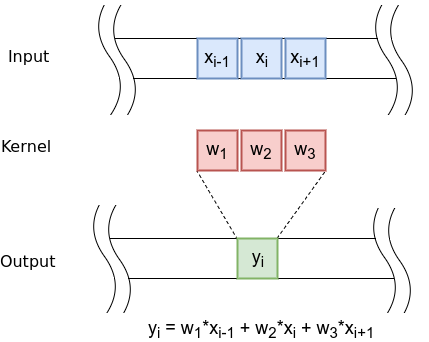
\includegraphics[width=0.5\textwidth]{./imgs/convolution.png}
		\caption{Convolution layer, kernel size 3 with with stride 1.}
		\label{fg:convolution}
	\end{center}
\end{figure}

\subsubsection{Activations}
After each convolution layer, usually nonlinear layer (know as activation layer) is applied. The purpose of this layer is to introduce nonlinearity to a system which consists of only linear operations as convolution layers are nothing more than just element-wise multiplications and summations. In classical neural networks, nonlinear functions like tanh and sigmoid were often used, but because of the undesirable property of saturation (at either end of 0 or 1 for sigmoid, -1 or 1 for tanh), other activations are more often used today with CNNs. 

ReLU. The Rectified Linear Unit has become very popular in the last few years. It computes the function f(x)=max(0,x). It is shown in \cite{NIPS2012_4824} that usage of ReLU greatly accelerates the convergence of stochastic gradient descent compared to the sigmoid or tanh activations. Calculation of ReLU is much also more efficient as it is is simply thresholding at zero. 

\begin{equation}
ReLU(x) =
\begin{cases}
x, & \text{if}\ x>0 \\
0, & \text{otherwise}
\end{cases} \\
\end{equation}


The downside of ReLU is still saturation to the 0 on one side. Once in this state, the neuron is unlikely to recover because the function gradient at 0 is also 0, so gradient descent learning will not alter the weights. This is the problem known as \textit{dying ReLU}.
Different variants of ReLU, PrRelu and ELU are often used to resolve this problem\cite{prelu}\cite{elu} with .  

\begin{equation}    
PrELU(x)=
\begin{cases}
x, & \text{if}\ x>0 \\
\alpha x, & \text{otherwise}
\end{cases}\\
\end{equation}
\begin{equation}
ELU(x)=
\begin{cases}
x, & \text{if}\ x>0 \\
\alpha (exp(x) - 1), & \text{otherwise}
\end{cases}    \\
\end{equation}

Figure \ref{fg:activations} shows different activation functions.
\begin{figure}[!htb]
	\begin{center}
		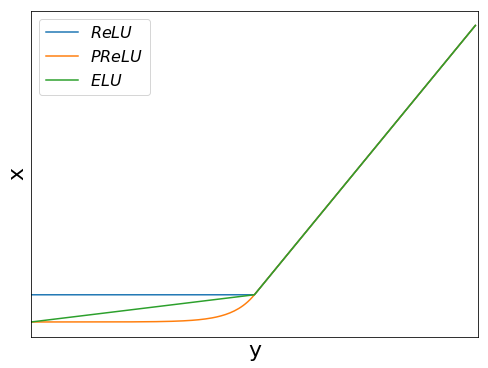
\includegraphics[width=0.5\textwidth]{./imgs/activations.png}
		\caption{Activation functions}
		\label{fg:activations}
	\end{center}
\end{figure}


\subsubsection{Pooling}

The pooling layer is usually placed after the convolutional layer. Its primary utility lies in reducing the spatial dimensions of the input for the next convolution layer while preserving the most salient information. Pooling also provides basic invariance to translation.

Similar to the convolution layer described previously, the pooling layer also uses sliding window or a certain size that is moved across the input transforming the values. Usually stride larger stride is used then in the convolution layers, as the purpose of this layer is subsampling. Most ofter, maximum value on the values in the window (max pooling) but other transformations are possible (average pooling, L2-norm, and even stochastic pooling).
Figure \ref{fg:pooling} show dimensionality reduction by factor 2 using pooling with kernel size 2 with stride 2.
\begin{figure}[!htb]
	\begin{center}
		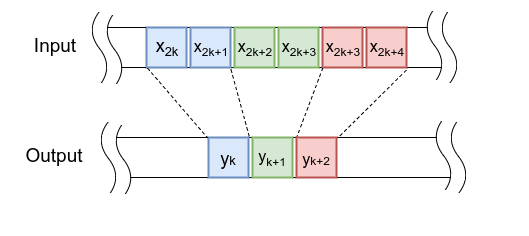
\includegraphics[width=0.5\textwidth]{./imgs/pooling.png}
		\caption{Dimensionality reduction by pooling (kernel size 2, stride 2)}
		\label{fg:pooling}
	\end{center}
\end{figure}




  
\subsubsection{Comparision with RNN}


During calculation, each \textit{patch} a convolutional kernel operates on is independent of the other meaning that the entire input layer can be processed concurrently which makes CNNs more efficient than RNNs. 

When compared with RNN, in which output can depend on the entire sequence, but in convolution layer, single output \textit{sees} only limited window in the previous layer defined by kernel size. This is called the receptive field of the convolution. 
Figure \ref{fg:receptive field} shows each new layers depends on larger portion of the input($z_i$ \textit{sees} 5 elements of input). 
This is the motivation behind deep convolution neural networks and why they are so popular in the field of image processing. Lower layers see limited spatial information and are able to detect simple features like edges and through a series of convolutional layers, later layers can detect more abstract concepts using intermediate features detected from the whole image, or the signal in our case.

\begin{figure}[!ht]
	\begin{center}
		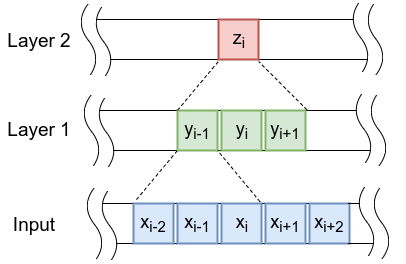
\includegraphics[width=0.5\textwidth]{./imgs/receptive_field.png}
		\caption{Receptive field after 2 layers of convolutions with kernel size 3}
		\label{fg:receptive field}
	\end{center}
\end{figure}
Stacking layers increases computational time as the input signal has to pass through the entire network but calculations at each layer can happen concurrently and each individual computation is small.
In practice, CNNs have a big speed up over RNNS. This especially goes when dealing with larger sequences\cite{facebook}.

During the forward pass, input flows and is transformed, hopefully becoming a representation that is more suitable for the task. During the back phase, the gradient is propagated back through the network. Just like in RNNs, this signal gets multiplied and depending on the scales it can vanish resulting in no gradient flow to lower layers and no parameter upgrades. This limits the depth of the network. Resnet arhitecture\cite{resnet} with its residual layers address this issue and allow deep architectures with steady gradient flow.




\subsection{Residual Networks}
A Residual Network or ResNet is a neural network architecture which solves the problem of vanishing gradients using the simple trick.  
Figure \ref{fg:resnet_block}  shows on the left classical CNN that takes input and transforms it using convolution layers and activations.  This can be represented as some nonlinear function $ H(x) $. $ H(x) $ can be written as a sum of other nonlinear function $F(X)$ and linear member $X$. $  F(X) $ is called the residual.

\begin{figure}[!ht]
	\begin{center}
		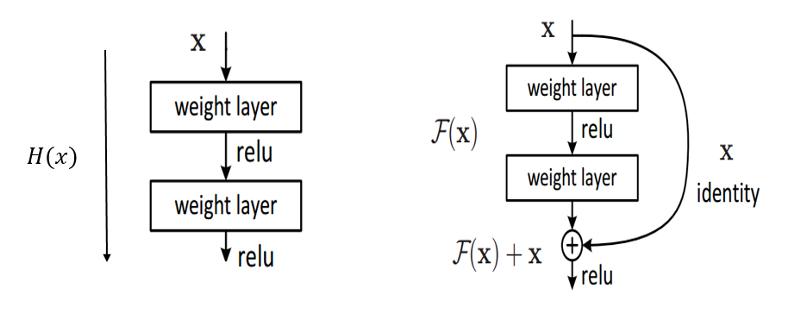
\includegraphics[width=0.7\textwidth]{./imgs/resnet_block.png}
		\caption[Comparison between classical CNN and CNN with residual connection ]{Comparison between classical CNN and CNN with residual connection \protect\footnotemark}
		\label{fg:resnet_block}
	\end{center}
\end{figure}
\footnotetext{Figure adapted from the original paper \cite{resnet}}
Instead of learning $H(X)$, network learns residual and at the output $x$ is simply summed up to the $F(x)$ as shown in the figure.  By stacking these layers, the gradient could theoretically \textit{skip} over all the intermediate nonlinear layers and reach the bottom without vanishing.




\section{CTC Loss}

The goal is to design model which can convert from a sequence of events of current measurements into a sequence of base pairs.

Suppose that we have an input sequence $X$ (signal data) and the desired output sequence $Y$ (nucleotides). $X$ and $Y$ will be of different lengths(the length of base pairs is always smaller than the length of the raw signal), which may pose a problem.

Instead of having a variable size of the output from the neural network, we can limit it to length $m$ and from direct output of the network in some way decode our desired output sequence $Y$. $m$ is the maximal allowed length of output sequence $Y$.
Idea is that the network outputs is fixed width and the variable length sequence is derived from them.
The neural network can be considered to be simply a function that takes in some input sequence $X$ (of length $n$) and generate some sequence $O$ (of length $m$). Note that this generated sequence is not same as output sequence $Y$. 

\subsection{Definition}
They key idea behind Connectionist Temporal Classification(CTC)\cite{Graves:2006:CTC:1143844.1143891} is that instead of directly generating output sequence $Y$ as output from the neural network, we  generate a probability distribution at every output length (from $t$=1 to $t$=$m$) that after \textit{decoding} gives maximum likelihood output sequence $Y$. 
Finally, network is trained by creating an objective function that restricts the maximum likelihood decoding for a given sequence $X$ to correspond to our desired target sequence $Y$.


Given an input sequence $X$ of length $n$, the network generates some probabilities over all possible labels (A, C, T, and G) with an extra symbol representing a "blank" at each timestep. 

The output generated by the network is called \textit{path}. Path is defined by the sequence of it's elements $\pi = (\pi_1, \pi_2, ..., \pi_m)$.
The probability of a given path $\pi$, given inputs $X$, can then be written as the product of all its forming elements:

\begin{equation}
\begin{gathered}
P(\pi | X) = \prod_{t=1}^{m} o_t(\pi_t), \\
\text{where $o_t(\pi_t)$ is probability of $\pi_t$ being $t^{th}$ element on path $\pi$}
\end{gathered}
\end{equation}

Real output sequence, for given path, is obtained by traversing the path and removing all blanks and duplicate letters. Let $ decode(\pi) $ be the output sequence corresponding to a path $\pi$. The probability of output sequence $Y$ is then the sum of probabilities of all paths that decode to $Y$:
\begin{equation}
\begin{gathered}
P(Y | X) = \sum_{\pi \in decode^{-1}(Y)}^{} P(\pi | X)
\end{gathered}
\end{equation}
\subsection{Objective}
Given the dataset $D = \{(X, Y)\}$, training objective is the maximization of the likelihood of each training sample which corresponds to the minimization of negative log likelihood:

\begin{equation}
\begin{gathered}
L(D) = - \sum_{(X,Y)\in D}^{} ln P(Y | X)
\end{gathered}
\end{equation}


\subsection{Output decoding}
Given the probability distribution $P(Y | X)$ and given input sequence $X$, most likely $Y^{*}$ can be computed.
\begin{equation}
\begin{gathered}
Y^{*} = \argmax_{Y \in L^m} P(Y|X) = \argmax_{Y \in L^m} \sum_{\pi \in decode^{-1}(Y)}^{} P(\pi | X),\\
\text{~where $L^m$ set of all possible sequences over alphabet $L$ }\\
\text{with length less than or equals to $m$}
\end{gathered}
\end{equation}

The probability of a single output sequence $Y$ is the sum of probabilities of all paths that decode to $Y$ and the most probable sequence is needed to be found.
Calculation of all possible sequences is computationally intractable but exist algorithms that approximate decoding. 

One naive possibility is to take the most probable path and say that output sequence corresponds to that path.
This is not necessarily true: suppose we have one path with probability $0.1$ corresponding with sequence $A$, and ten paths with probabilities  $0.05$ each corresponding to sequence $B$. Clearly, label $B$ is preferable overall, since it has an overall probability of $0.5$; however, this naive best path decoding would select label $A$, which has a higher probability than any single path for label $B$.

Better approximations can be calculated using beam search algorithm proposed in paper\cite{graves_decode}.  
Idea behind this approach is tu 

This serves as a brief overview of the method and explains key concepts why it is used. More detailed explanation can be found in original paper\cite{Graves:2006:CTC:1143844.1143891} or various blog post\cite{ctc-blog}.

\section{Batch normalization}
Batch normalization is method proposed in paper\cite{BNORM} that accelerates learning process. 
During training parameters are updated and distribution of outputs of each layers keep changing. Small change in distribution of outputs in early layers can cause drastic change in later layers and those layers need to adapt to the new scale of their inputs. This change of distribution is called the internal covariate shift and results in slows learning.
Proposed solution for this is to center each output from activations of the mini-batch to zero-mean and unit variance. After that learned scale and offset are applied. This process is called batch normalization. 
After training, mean and variance for each activation is computed on the whole training dataset rather than on mini-batches during training. 
Pros of using batch normalization 
Batch normalization offers several advantages other than reducing internal covariant shift. 
If offers more robust learning process by reducing dependance on scale of the parameters and their initial values. This allows usage of larger learning rates and faster learning all together. It is show in the original paper that batch normalisation also regularizes the model that could potentially improve performance of the model.

%%%%%%%%%%%%%%%%%%%%%%%%%%%%%%%%%%%%%%%%%%%%%%%%%%%%%%%%%%%%%%%%%%%%%%%%%%%%%%%%%%%%%%%
%% CHAPTER
\chapter{Implementation}

\section{Datasets}

Datasets show in table ref are used. Ecoli as a sample of larger number of reads and lambda as a small example used for testing purposes. Both datasets were previously have passed to MinKNOW and have been basecalled by Metrichor.
Baseced data by Metrichor are used to train our model.
\begin{savenotes}
\begin{table}[htb]
	\caption{Used datasets}
	\label{tbl:datasets}
	\centering
	
	\begin{tabular}{lcc| c}
		\toprule
		{} &  \thead{Number of reads} &   \thead{Total bases (bp)\footnote{Total number of bases calle by Metrichor}} &    \thead{Whole genome size (bp)} \\
		\midrule
		\textit{{E. Coli}}\footnote{R9 sequencing data from \url{http://lab.loman.net/2016/07/30/nanopore-r9-data-release/}, reference taken from \url{https://www.ncbi.nlm.nih.gov/nuccore/48994873}} & 164471 & 1 481 687 490 & 4 639 675\\
		\textit{lambda}\footnote{Internal dataset, reference taken from \url{https://www.ncbi.nlm.nih.gov/nuccore/NC_001416.1}}   & 86 &  466 465 & 48 502  \\

		\bottomrule
	\end{tabular}
\end{table}
\end{savenotes}


 Figure \ref{fg:events} show data preset in FAST5 file after basecalling by Metrichor. For basecalled event, $model\_state$ field contains possible sequence of bases in the pore and $move$ field defines by how many bases have passed through the pore between two consequitive events. 


\begin{figure}[!ht]
	\begin{center}
		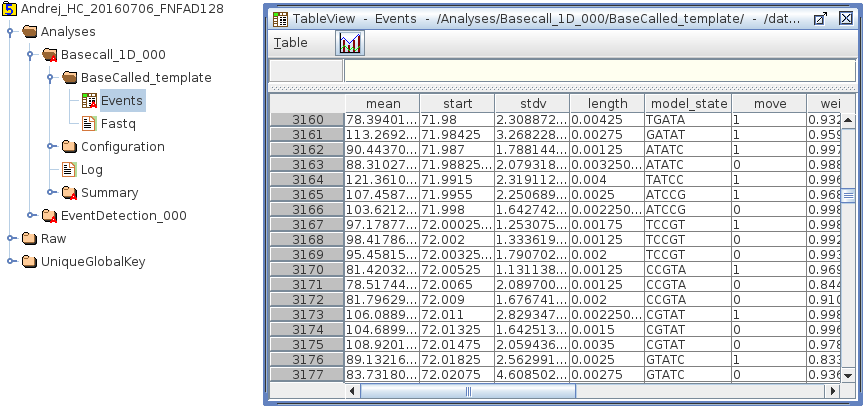
\includegraphics[width=1\textwidth]{./imgs/basecall_events.png}
		\caption{Basecall information produced by Metrichor show in HDFView}
		\label{fg:events}
	\end{center}
\end{figure}

\section{Technologies}

Overall solution was implemented in Python programing language. Described model is implemented using TensorFlow. It is an open source software library for numerical computation using data flow graphs developed by Google. TensorFlow, even though is considered low-level framework, offers implementations of many higher level concepts (layers, losses, and optimizers) which makes it great for prototyping while keeping it modular and extensible for highly specific tasks as well.

TensorFlow offers efficient GPU implementations of various layers and losses but as of version 1.2 lacks GPU implementation of used CTC loss, so WARP-CTC\footnote{\url{https://github.com/baidu-research/warp-ctc}} was used. It offers both GPU and CPU implementations as well as bindings for TensorFlow.

For alignment tasks, developed tool offers support for GraphMap and BWA but can easily be extended with any other aligner that outputs results in same file format (SAM).

SAMTools\footnote{\url{http://www.htslib.org/}} and it's Python bindings PySam\footnote{\url{https://github.com/pysam-developers/pysam}} were used for conversions between various file formats used in Bioinformatics.

Docker was used for automating the deployments on different machines. It helps us resolve problem know as \textit{dependency hell}\footnote{\url{https://en.wikipedia.org/wiki/Dependency_hell}}  keeping all dependencies in single container thus eliminating possible conflict between packages on host OS.
Nvidia Docker\footnote{\url{https://github.com/NVIDIA/nvidia-docker}} was used for GPU support.


Training and all evaluations were done on the server with  \textit{Intel(R) Xeon(R) E5-2640 CPU}, 600 GB of RAM and \textit{NVIDIA TITAN X Black} with 6GB of GDDR5 memory and 2880 CUDA cores.

All developed and used code, including utility scripts is publicly available on \textit{GitHub}\footnote{\url{https://goo.gl/RVeyjU}} under the \textit{MIT Licence}.

\section{File formats}
This section will give brief overview of file formats used and information present in them.
\subsubsection{FASTA}


FASTA is widely used file format for reference sequences. It is a text-based format for representing either sequences, in which nucleotides or amino acids are represented using single-letters. Most usual file extensions are \textit{.fasta} or \textit{.fa}).
Sequence representation consists of header line containing description starting with character $ > $, folowed followed by line(s) of sequence data. Full file specification can be found at \textit{NCBI} sited\footnote{\url{http://www.ncbi.nlm.nih.gov/BLAST/blastcgihelp.shtml}}.
 Figure \ref{fg:fsta} shows example of sequence stored in FASTA file format.
\begin{figure}[!ht]
	\begin{center}
		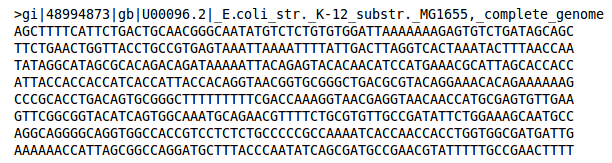
\includegraphics[width=0.8\textwidth]{./imgs/fasta.png}
		\caption{Example of FASTA file}
		\label{fg:fsta}
	\end{center}
\end{figure} 

\subsubsection{FASTQ format}
Reads are usualy stored in FASTQ file format. Each read in the file is stored in followig way:
\begin{enumerate}
	\item character "$@$" followed  by a sequence identifier and an optional description 
	\item sequence
	\item character "$+$" character and is optionally followed by the same sequence identifier and description.
	\item quality score for each base
\end{enumerate}
Quality score is generated during basecalling that can be used by aligners. Quality is represented by ASCII printable characters where
the character "$!$" represents the lowest quality while "\textasciitilde" is the highest. Figure \ref{fg:fq} shows example of read stored in FASTQ file format.
\begin{figure}[!ht]
	\begin{center}
		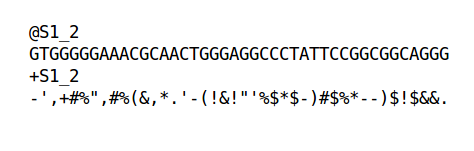
\includegraphics[width=0.6\textwidth]{./imgs/fq.png}
		\caption{Example of FASTQ file}
		\label{fg:fq}
	\end{center}
\end{figure} 

\subsubsection{SAM format}
The Sequence Alignment/Map (SAM) format is a generic format for storing
reads alignments against reference sequences. It is a TAB-delimited text format consisting
of header section, which is optional, and an alignment section. Detailed information about SAM specification can be found on \textit{SAMTools} website\footnote{\url{https://samtools.github.io/hts-specs/SAMv1.pdf}}.
Among other information, alignment start position is included, flag stating is read aligned as template of as reverse complement and CIGAR string that describes alignment.
 Figure \ref{fg:align} shows simple alignment and CIGAR string. 
There are several possible letters that can appear in CIGAR string but most importantly matches, mismatches, insertions and deletions are represented with letters "=", "X", "I" and "D".

 
\begin{figure}[!ht]
	\begin{center}
		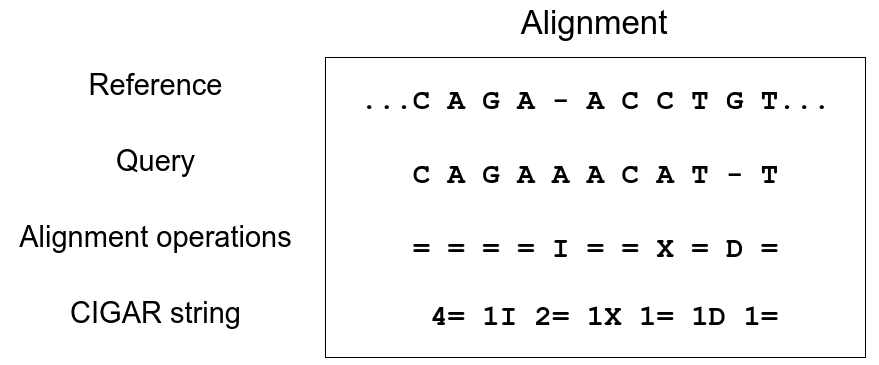
\includegraphics[width=0.6\textwidth]{./imgs/alignment.png}
		\caption{Example of simple alignment and CIGAR string}
		\label{fg:align}
	\end{center}
\end{figure} 


\section{Data preprocess}


To help training process, raw signal is split into smaller blocks (signals of length 1000) that are used as inputs. For Metrichor basecalled event using $start$ field it is easy to calculate the block it falls into. With this, for each block we have output by Metrichor. 
To correct errors produced by Metrichor and possibly increase quality of data, each read aligned to the reference using aligner GraphMap thet returns best position in the genome, hopefully the part of the genome from which read came from.
Alignment part in the genome is used as target. Using cigar string returned by aligner we can correct Metrichor data and with that our test data per blocks. This process is shown in figure \ref{fg:data_correction}.

\begin{figure}[!ht]
	\begin{center}
		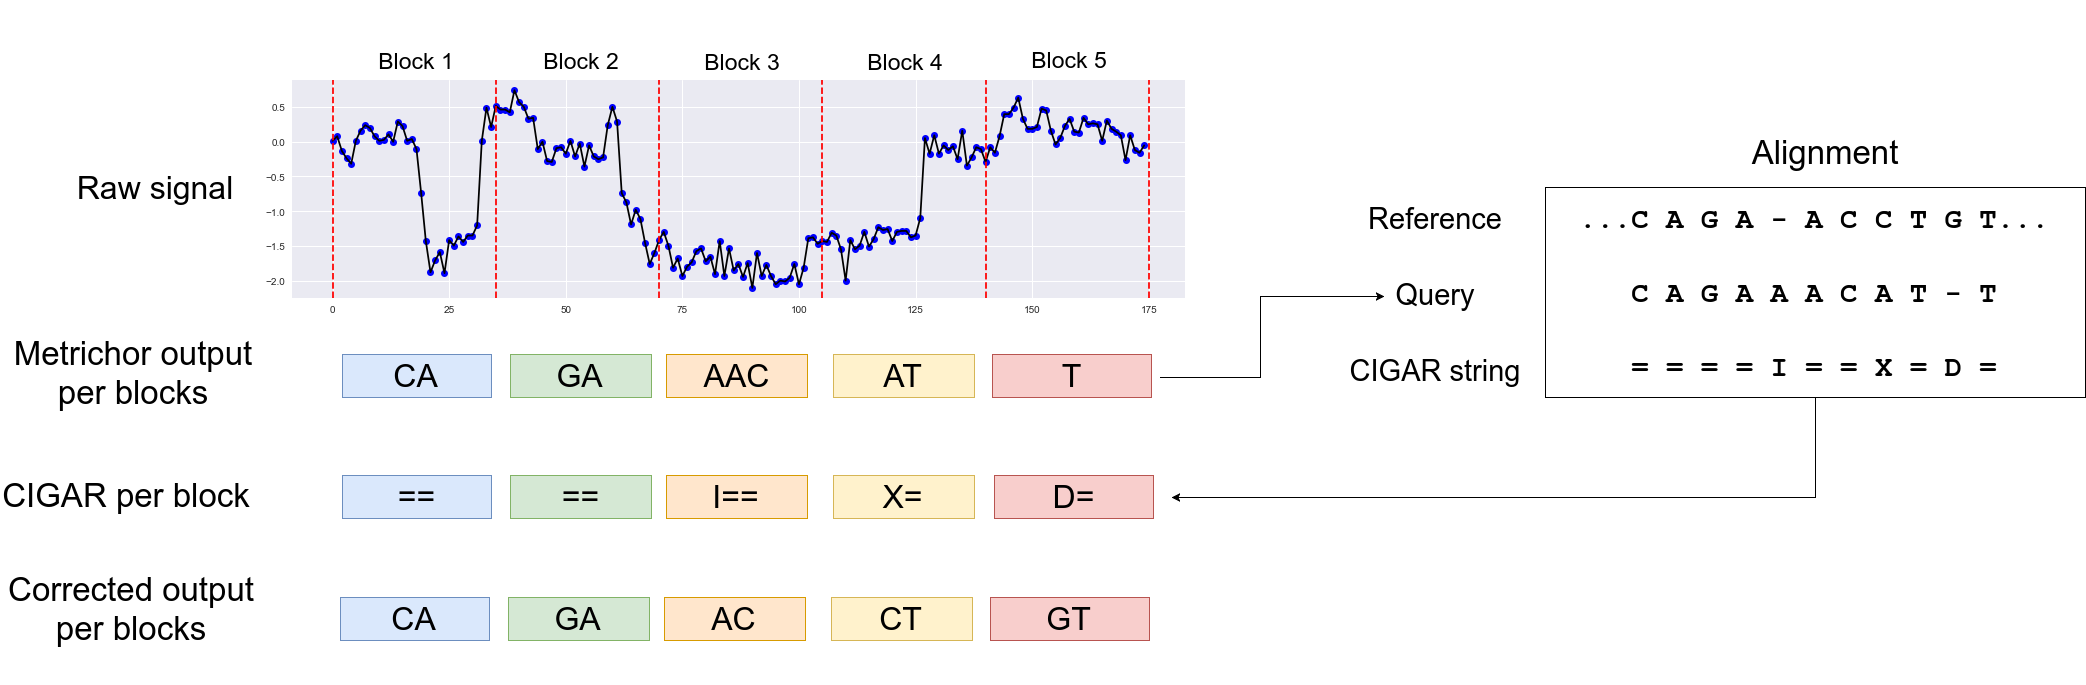
\includegraphics[width=1\textwidth]{./imgs/train_data_correction.png}
		\caption{Dataset preparation}
		\label{fg:data_correction}
	\end{center}
\end{figure}


To eliminate possibility of overfitting to the know reference, model is trained and tested on reads from different organisms. Due to limited ammount of public available nanopore sequence data, ecoli was \textit{devided} into two regions.
Reads were split into into train and test portions depending in which region of ecoli they align to. 
If read aligns inside first 70\% of the ecoli it is placed into train set and if it aligns in second portion it is placed into test set. Reads whose aligment overlaps train and test region are not used. Important to note that ecoli,and genome of majority of other bacteris, has cyclical genome so reads with alignment that wraps over edges are also discarded. Total train set consist of bla bla reads.
Overview of the entire learning pipeline is shown in figure \ref{fg:train_pipe}.
\begin{figure}[!ht]
	\begin{center}
		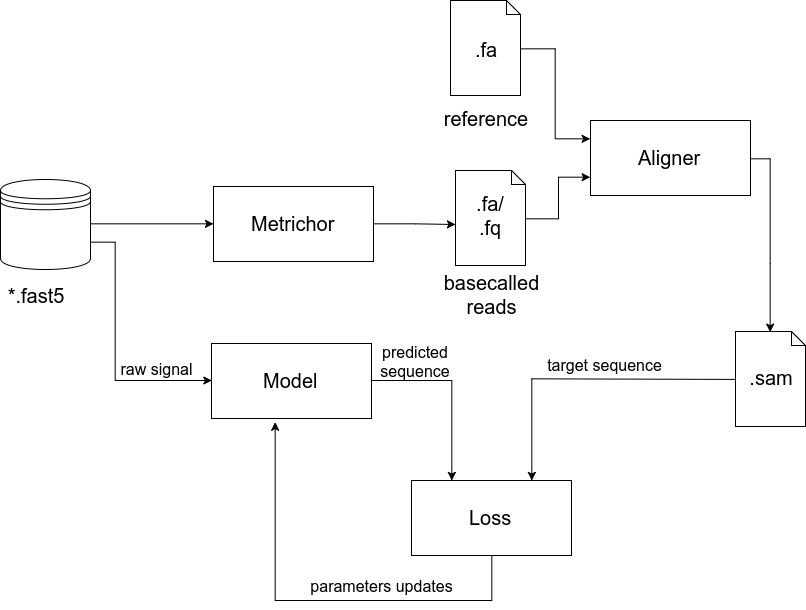
\includegraphics[width=0.7\textwidth]{./imgs/train_pipeline.png}
		\caption{Overview of training pipeline}
		\label{fg:train_pipe}
	\end{center}
\end{figure}
\section{Deep Learning model}

Final model is residual neural network consisting of 72 residual blocks depicted in figure \ref{fg:model_block}. This is a variant of arhitecture proposed in paper \cite{identitet} with the difference of ELU being used as activation instead of ReLU as it is reported\cite{resnet-elu} to speeds up learning process and improve accuracy as the depth increase. 
without running more detailed analysis is difficult if this this actually results in performance benefit over simple ReLU .

Each residual block contains 2 convolution layers making total number of convolution layers 144. Each convolutional layer in this models uses 64 kernels of 3. Because  sequenced read is always shorter than the raw signal, pooling with kernel size 2 is used every 48 layers resulting in reduction of dimensionality by factor 8. This is used to help training by reducing number of required blank labels in the output and computation effort. This network has 2 milion peremeters that are learned during training. 


\begin{figure}[!ht]
	\begin{center}
		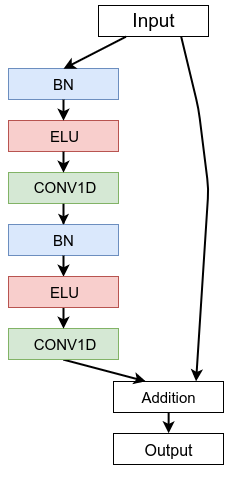
\includegraphics[width=0.2\textwidth]{./imgs/model.png}
		\caption{Used residual block}
		\label{fg:model_block}
	\end{center}
\end{figure}


Training the model is minimization of previously described CTC loss. It was done using Adam, stochastic gradient descent algorithm based on estimation of 1st and 2nd-order moments.
It is often used as it offers fast and stable convergention. Default parameters of Adam were used (
$\beta_1=0.9$ and $\beta_2=0.999$. Initial earning was set to 1e-3 with exponential decay. Batch size was set to 8 mostly due to limited hardware resources. As noisy batch that would cause gradients to explode, gradient is clipped to range [-2, 2].
Figure \ref{fg:learn} shows learning curves during training. Occasional spikes of training loss be explained small batch size and presence of noise in the signal. 

\begin{figure}[!ht]
	\begin{center}
		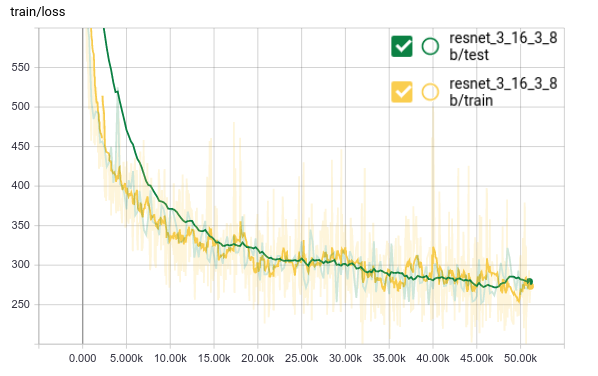
\includegraphics[width=0.6\textwidth]{./imgs/train_tb.png}
		\caption{Learning curve shown in TensorBoard}
		\label{fg:learn}
	\end{center}
\end{figure}

Training process is implemented in \textit{producers/consumer} pattern with synchronization and communication done using FIFO\footnote{FIFO is an acronym for first in, first out} queue. Multiple producer threads, running on the CPU, load FAST5 and aligments batch data, preprocess it and convert to Tensorflow objects, while single GPU worker takes batch from the queue and computes forwards and backward passes on the network. This is done to reduce time between batches and maximize GPU utilization during training. 












%TODO REZULTATI
%%%%%%%%%%%%%%%%%%%%%%%%%%%%%%%%%%%%%%%%%%%%%%%%%%%%%%%%%%%%%%%%%%%%%%%%%%%%%%%%%%%%%%%
%% CHAPTER
\chapter{Results}
Developed was compared with other available basecallers that support R9 chemisty. This includes third-party basically DeepNano and official basecallers by Oxford Nanopore (cloud-based Metrichor and NanoNet).
Fact that ground truth is not actually known makes evaluation difficult. Two approaches were used to get clearer information about each basecaller.
In all tables and figures, developed model is addressed as \textit{resdeep} simply due to fact it is deep residual neural network.



\section{Error rates per read}

Basecalled reads are aligned to the reference using GraphMap and alignments are analyzed. If the whole sequencing is done correctly and quality basecaller is used, all reads should align to the reference. Missmatches, insertions and deletions, in that case, should be due to limitations of sequencing technology and noise in the signal.

To get conclusive results this is done on both test set of the ecoli dataset as well as lambda dataset. 
A portion of the read length that aligns as correctly is called match\_rate. Same goes for mismatches and insertions. 
Sum of all matches, mismatches, and insertions is equal to the reads length \ref{eq:read_len}. Deletions are not part of the read as they are the absence of base that occurs in the reference. Deletion\_rate is defined as a number of deletions in the alignment over the length of the aligned read. All expressions can be found bellow.

\begin{equation}
\begin{gathered}
\label{eq:read_len}
read\_len =  n\_matches + n\_missmatches + n\_insertions 
\end{gathered}
\end{equation}
\begin{equation}
\begin{gathered}
match\_rate = \dfrac{n\_matches}{read\_lenght}
\end{gathered}
\end{equation}
\begin{equation}
\begin{gathered}
missmatch\_rate = \dfrac{n\_missmatches}{read\_lenght}
\end{gathered}
\end{equation}
\begin{equation}
\begin{gathered}
insertion\_rate = \dfrac{n\_insertions}{read\_lenght}
\end{gathered}
\end{equation}
\begin{equation}
\begin{gathered}
deletion\_rate = \dfrac{n\_deletion}{read\_lenght}
\end{gathered}
\end{equation}
\begin{equation}
\begin{gathered}
match\_rate = \dfrac{n\_matches}{read\_lenght}
\end{gathered}
\end{equation}


For each basecaller, these rates are expressed as median, mean and variance of all aligned reads. To summarize the results, the median is used as a single value as it is more robust measure and in the case of skewed distributions like these even more informative.  Results are show in the table \ref{tbl:ecoli_rates} for ecoli dataset and table \ref{tbl:lambda_rates} for lambda. 
Developed model show promising results by having better match rate than the others, smaller mismatch rate. Both dataset show all basecallers being a bit bias towards deletions than insertions but this can be bias of aligner used (GraphMap). To eliminate that possibility, tests were repeated with BWA with almost same results. Results for BWA are show in tables
\ref{tbl:ecoli_rates_bwa} and \ref{tbl:lambda_rates_bwa}.
All results are consistent on both datasets using both aligners.





\begin{table}[htb]
	\caption{Alignment specifications of Ecoli R9 basecalled reads}
	\label{tbl:ecoli_rates}
	\centering
	\begin{tabular}{lcccc}
		\toprule
		{} &  \thead{Match \% \\(median)} &  \thead{Mismatch \% \\(median)} &  \thead{Insertion \% \\(median)} &  \thead{Deletion \% \\(median)} \\
		\midrule
		
		deepnano   &                  90.254762 &                      6.452852 &                       \textbf{3.274420} &                     11.829965 \\
		metrichor  &                  90.560455 &                      5.688105 &                       3.660381 &                      8.328271 \\
		nanonet    &                  90.607674 &                      5.608912 &                       3.652791 &                      8.299046 \\
		resdeep    &                  \textbf{91.408591} &                     \textbf{ 5.019141} &                       3.477739 &                      \textbf{7.471608 }\\
		\bottomrule
	\end{tabular}
\end{table}

\begin{table}[htb]
	\caption{AlignmenBWAA t specifications of Ecoli R9 basecalled reads}
	\label{tbl:lambda_rates_bwa}
	\centering
	\begin{tabular}{lcccc}
		\toprule
		{} &  \thead{Match \% \\(median)} &  \thead{Mismatch \% \\(median)} &  \thead{Insertion \% \\(median)} &  \thead{Deletion \% \\(median)} \\
		\midrule
		deepnano   &                  90.254762 &                      6.452852 &                       3.274420 &                     11.829965 \\
		metrichor  &                  90.595441 &                      6.869543 &                       2.531646 &                      7.567381 \\
		nanonet    &                  90.988989 &                      6.674760 &                     \textbf{  2.348552} &                      7.698530 \\
		resdeep    &                 \textbf{ 91.470588} &                      \textbf{5.929204 }&                       2.477283 &                     \textbf{ 6.970362} \\
		\bottomrule
	\end{tabular}
	
\end{table}
\begin{table}[htb]
	\caption{Alignment specifications of lambda R9 basecalled reads}
	\label{tbl:lambda_rates}
	\centering
	\begin{tabular}{lcccc}
		\toprule
		{} &  \thead{Match \% \\(median)} &  \thead{Mismatch \% \\(median)} &  \thead{Insertion \% \\(median)} &  \thead{Deletion \% \\(median)} \\
		\midrule
		deepnano   &                  86.997687 &                      9.623494 &                       3.442490 &                     16.052830 \\
		metrichor  &                  87.714988 &                      7.835052 &                       4.093851 &                     \textbf{10.757491} \\
		nanonet    &                  88.415611 &                      8.178372 &                       3.629653 &                     11.793022 \\
		resdeep    &                 \textbf{ 89.694482} &                     \textbf{ 7.238095} &                       \textbf{3.078796} &                     13.450292 \\
		\bottomrule
	\end{tabular}




\end{table}
\begin{table}[H]
	\caption{Alignment specifications of bwa lambda R9 basecalled reads}
	\label{tbl:lambda_rates}
	\centering
	\begin{tabular}{lcccc}
		\toprule
		{} &  \thead{Match \% \\(median)} &  \thead{Mismatch \% \\(median)} &  \thead{Insertion \% \\(median)} &  \thead{Deletion \% \\(median)} \\
		\midrule
		
		deepnano   &                  86.625973 &                     11.288361 &                       2.098225 &                     14.648308 \\
		metrichor  &                  87.294093 &                     10.109186 &                       2.376476 &                      \textbf{9.645323 }\\
		nanonet    &                  87.767037 &                     10.017598 &                       2.354248 &                     10.597232 \\
		resdeep    &                 \textbf{ 89.049870} &                     \textbf{ 9.480883} &                       \textbf{1.615188 }&                     12.962441 \\
		\bottomrule
	\end{tabular}
	
\end{table}


Distribution of these rates are shown using  histogram plot on figure \ref{fg:hist} and the KDE (kernel density estimate) plot (figures \ref{fg:ecoli_kde} and \ref{fg:lambda_kde}). Like the histogram, the KDE plot encodes the density of observations, but curve approximation is used instead of bins. This results in less cluttered comparison. 
histogram plots for lambda are show on plot \ref{fg:lambda_hist}. It is important to note that lambda is small dataset (around 80 reads) and more samples are needed to get a better approximation of distribution.

\begin{figure}[!htb]
	\begin{center}
		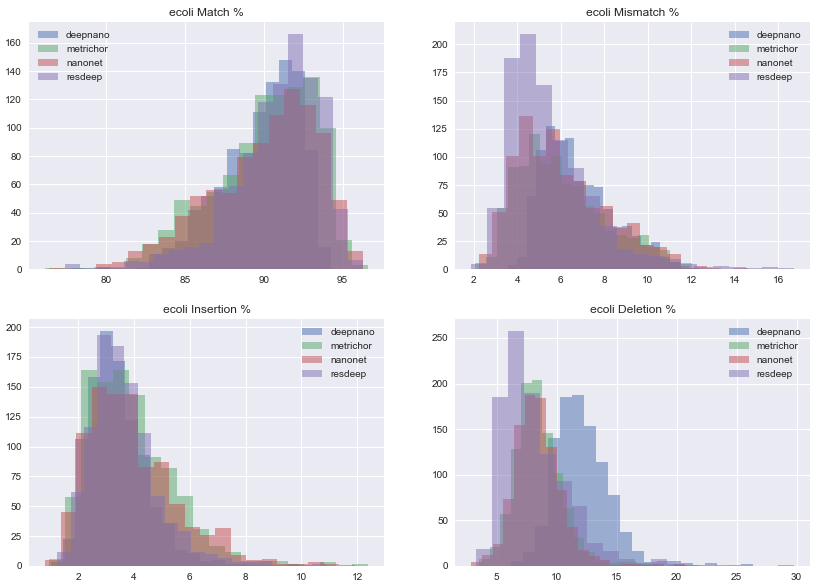
\includegraphics[width=0.8\textwidth]{./imgs/results/ecoli/hist_20.png}
		\caption{Cigar operations histogram over relative position inside read}
		\label{fg:hist}
	\end{center}
\end{figure}

\begin{figure}[!htb]
	\begin{center}
		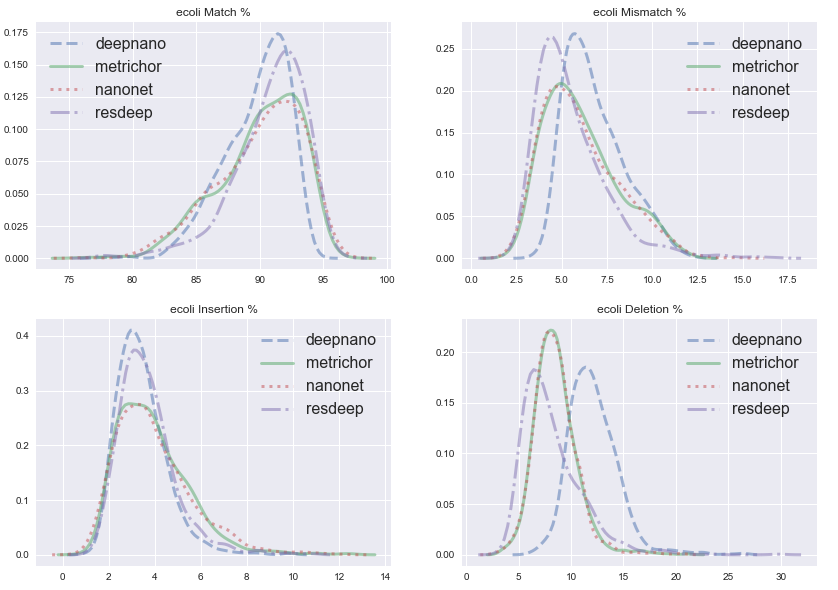
\includegraphics[width=0.8\textwidth]{./imgs/results/ecoli/kde_cigar_lines.png}
		\caption{Cigar operations histogram over relative position inside read}
		\label{fg:ecoli_kde}
	\end{center}
\end{figure}

\begin{figure}[!htb]
	\begin{center}
		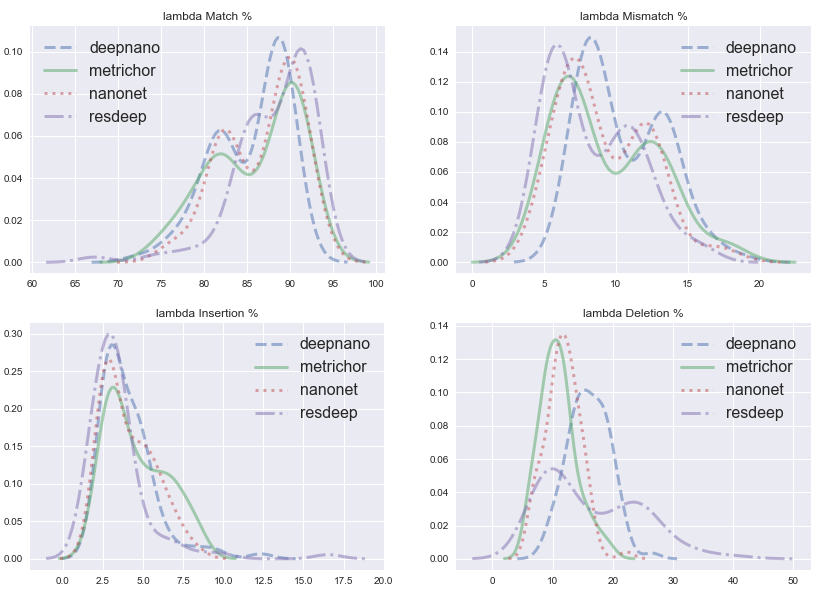
\includegraphics[width=0.8\textwidth]{./imgs/results/lambda/kde_cigar_lines.png}
		\caption{Cigar operations histogram over relative position inside read}
		\label{fg:lambda_kde}
	\end{center}
\end{figure}


Histogram on figure \ref{fg:cigar_op_dist} shows how matches, mismatches, insertions, and deletions are distributed across the reads. It is shown that mismatches and insertion occur more frequently at the ends. This is not only the case for the developed basecaller, but other basecallers show same property. This could be because context information is not available from both sides when edges are base called.

\begin{figure}[!ht]
	\begin{center}
		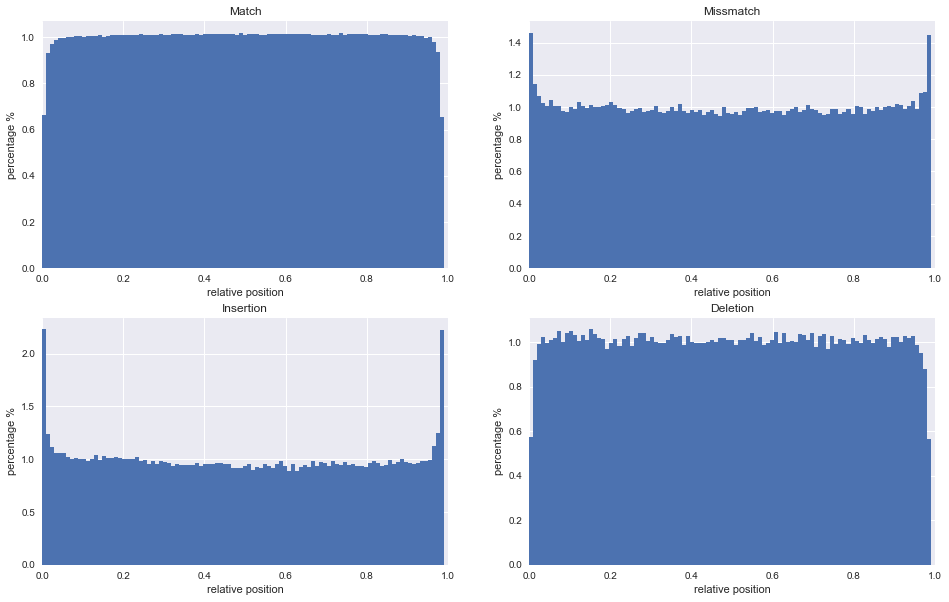
\includegraphics[width=1\textwidth]{./imgs/operation_distributed_r9.png}
		\caption{Cigar operations histogram over relative position inside of read}
		\label{fg:cigar_op_dist}
	\end{center}
\end{figure}





\section{Consensus}

Only aligning the reads to the reference and calculating described error rates and match rates per read could be misleading as it is simple to produce a naive model that obtains excellent results. Let us consider a model that basecalls single base "A" for every input signal. Aligning "A" to the reference (supposing that the aligner doesn't discard short and highly ambiguous reads) will always return perfect alignment as certainly nucleotide "A" is present in the reference. This model has perfect match rate with non-existent missmatches, insertions, and deletions.  The second approach is used, in addition to the first, to give a more rigorous comparison.

Idea is to check if the reconstruction of the reference is possible from the reads and how closely does it match the original reference. Instead of going through the whole assembly process, as we know the reference genome of the data used in these tests, we simply align all the reads to the genome, stack them on top of each other forming pileup of read bases. Using majority vote bases are called on each position. The resulting sequence is called consensus. When calling consensus for deletions,  there has to be a majority of deletions of the same length. Calling insertions has the additional condition and majority has to agree on both length and the inserted bases. Figure \ref{fg: consensus} shows how consensus is called from pileup created from aligned reads. Pileup is stored in mpileup format.  
Percentage of covered base is calculated to show much of reference genome is covered by at least one read. Similarly as before, match rate, mismatch rate, insertion and deletion rates are calculated but this time for whole consensus sequence. 


\begin{equation}
\begin{gathered}
identity\_percentage =  100 * \dfrac{n\_correct\_bases}{reference\_lenght}
\end{gathered}
\end{equation}
\begin{equation}
\begin{gathered}
match\_rate = \dfrac{n\_correct\_bases}{consensus\_lenght}
\end{gathered}
\end{equation}
\begin{equation}
\begin{gathered}
snp\_rate = \dfrac{n\_snp}{consensus\_lenght}
\end{gathered}
\end{equation}
\begin{equation}
\begin{gathered}
insertion\_rate = \dfrac{n\_insertions}{consensus\_lenght}
\end{gathered}
\end{equation}
\begin{equation}
\begin{gathered}
deletion\_rate = \dfrac{n\_deletion}{consensus\_lenght}
\end{gathered}
\end{equation}

Results are shown in the table. 
For ecoli, developed model shows results promising results comparable, if not better, with Metrichor in all aspects (matches, mismatches, insertions, and deletions). Lambda test shows that the results of the developed model fairly matches Metrichor. 



\begin{figure}[!ht]
	\begin{center}
		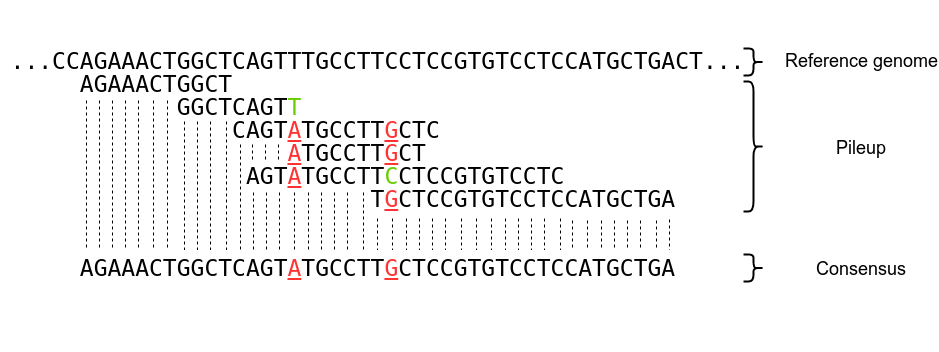
\includegraphics[width=0.8\textwidth]{./imgs/consnesus.png}
		\caption{Consensus from pileup}
		\label{fg:consensus}
	\end{center}
\end{figure}




\begin{table}[htb]
	\caption{Consensus specifications of Ecoli R9 basecalled reads}
	\label{tbl:spec}
	\centering

\begin{tabular}{lcccccc}
	\toprule
	{} &  \thead{Total called\\(bp)} &  \thead{Correctly called\\(bp)} &  \thead{Match\\\%} &  \thead{Snp\\\%} &  \thead{Insertion\\\%} &  \thead{Deletion\\\%} \\
	\midrule
	deepnano  &                  1510244.0 &                      1493242.0 &          98.8742 &         1.0044 &               0.1214 &              0.9041 \\
	metrichor &                  1515893.0 &                      1502588.0 &          99.1223 &         0.7464 &               0.1313 &              0.6300 \\
	nanonet   &                  1414237.0 &                      1385515.0 &          97.9691 &         1.5700 &               0.4609 &              1.5158 \\
	resdeep   &                  1517828.0 &                      1506233.0 &          \textbf{99.2361} &         \textbf{0.6474} &               \textbf{0.1165} &             \textbf{ 0.5510 }\\
	\bottomrule
\end{tabular}

\end{table}

\begin{table}[htb]
	\caption{Consensus specifications of lambda R9 basecalled reads}
	\label{tbl:spec}
	\centering

\begin{tabular}{lcccccc}
	\toprule
	{} &  \thead{Total called\\(bp)} &  \thead{Correctly called\\(bp)} &  \thead{Match\\\%} &  \thead{Snp\\\%} &  \thead{Insertion\\\%} &  \thead{Deletion\\\%} \\
	\midrule
	deepnano  &                    48342.0 &                        48025.0 &          99.3443 &         0.6433 &               \textbf{0.0124} &              0.2648 \\
	metrichor &                    48469.0 &                        48257.0 &          \textbf{99.5626} &         \textbf{0.4188} &               0.0186 &              \textbf{0.1465} \\
	nanonet   &                    48438.0 &                        48168.0 &          99.4426 &         0.5409 &               0.0165 &              0.1961 \\
	resdeep   &                    48385.0 &                        48163.0 &          99.5412 &         0.4402 &               0.0186 &              0.1976 \\
	\bottomrule
\end{tabular}
\end{table}

All model show slight bias towards deletions than insertions but this may actually be limitation of technology it is reported that deletion and mismatch rates for nanopore data are generally higher than insertion rates\cite{graphmap}.





\section{Read lengths}
Interesting thing to analyze are the lengths of basecalled reads for each tool. Developed tool output reads of lengths similar to metrhihor while other tools such as NanoNet for instance, basecall drastically shorter reads. More detail analysis of read length distributions is show using KDE plots on figure \ref{fg:r_lens} for both lambda and ecoli.



\begin{table}[htb]
	\caption{Ecoli R9 basecalled read lengths in base pairs}
	\label{tbl:ecoli_lens}
	\centering
	
	\begin{tabular}{lccc}
		\toprule
		{} &  \thead{median} &   \thead{mean} &    \thead{std} \\
		\midrule
		deepnano   &        5526.5 &  8126.694000 &  7406.554786 \\
		metrichor  &        5809.5 &  8933.275000 &  9189.709720 \\
		nanonet    &        3286.5 &  4874.406582 &  4803.182344 \\
		resdeep    &        5784.0 &  8990.988989 &  9297.972688 \\
		\bottomrule
	\end{tabular}
\end{table}


\begin{table}[htb]
	\caption{lambda R9 basecalled read lengths in base pairs}
	\label{tbl:ecoli_lens}
	\centering
	
	\begin{tabular}{lccc}
		\toprule
		{} &  \thead{median} &    \thead{mean} &    \thead{std} \\
		\midrule
		deepnano   &        4740.0 &   4664.750000 &  2628.512543 \\
		metrichor  &        5491.0 &   5482.952941 &  2748.446253 \\
		nanonet    &        4931.5 &   4925.804878 &  2739.987512 \\
		resdeep    &        5229.0 &   5138.764706 &  2605.958080 \\
		\bottomrule
\end{tabular}
\end{table}

	\begin{figure}[!ht]
		\begin{center}
			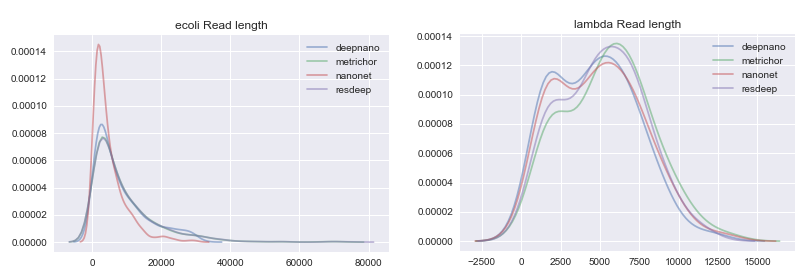
\includegraphics[width=1\textwidth]{./imgs/lens.png}
			\caption{Overview of evaluation pipeline}
			\label{fg:r_lens}
		\end{center}
	\end{figure}

\section{Speeds}
deep network with milions of parameters and 144layers

\subsection{Evaluation pipeline}
Entire evaluation pipeline is shown in figure \ref{fg:eval_pipe}. For aligment purposes GraphMap. Convertion between SAM and its binary variant BAM as well as generation of mpileup was done using SAMTools.
\begin{figure}[!ht]
	\begin{center}
		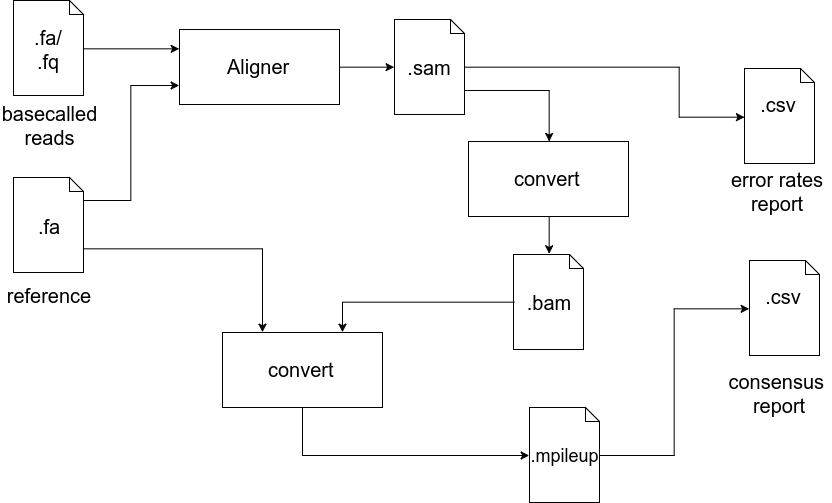
\includegraphics[width=0.7\textwidth]{./imgs/evaluation_pipeline.png}
		\caption{Overview of evaluation pipeline}
		\label{fg:eval_pipe}
	\end{center}
\end{figure}

%TODO ZAKLJUCAK
%%%%%%%%%%%%%%%%%%%%%%%%%%%%%%%%%%%%%%%%%%%%%%%%%%%%%%%%%%%%%%%%%%%%%%%%%%%%%%%%%%%%%%%
%% CHAPTER
\chapter{Conclusion}
Conclusion.

The main reason you might want to consider convolutions in your work is because they are fast. I think that’s important to make research and exploration faster and more efficient. Faster networks shorten our feedback cycles.

Most of the tasks I’ve encountered with text end up having the same requirement of the architecture: Maximize the receptive field while maintaining an adequate flow of gradients

When I set out to write this I only had my own experience and Google’s ByteNet to back this claim up. Just this week, Facebook published their fully convolutional translation model and reported a 9X speed up over LSTM based models.






On all tests developed model show excellent results. To prove this, this model needs to be tested on larger datasets from different sequencing runs of various organisms.


All test are done on data for R9 chemistry. Separate model using same architecture and loss can be trained on newer data.  Publicly available data R9.4 can be found here. It would be interesting to see how well can this approach compare to other reacently released models by Oxford Nanopore.

R9.5 data and new 1D2 reads are just becoming available. 


Metrichor was only available basecaller and was offered as a cloud service. Without added support for newer sequencing data, this model has limited application. It can be used as a demonstration of a different approach to base calling which yields promising results. 
As newer versions of basecallers by Oxford Nanopore do not support for data sequenced with older chemistry, this tool could be used to re-basecall all sequencing data and possibly improve results in some application.

Future work involves training on publicly available R9.4 data (loman)(zika) and R9.5 when it becomes available. Possible improvements of the model include the combination of convolutions and attention mechanism proposed just recently in the paper that shows excellent results in both speed and accuracy in tasks of language translation. SELU je jako jeben za probat jos isto that makes Batch normalization layer obsolete[link]. 



%TODO ABSTRACTS
%%%%%%%%%%%%%%%%%%%%%%%%%%%%%%%%%%%%%%%%%%%%%%%%%%%%%%%%%%%%%%%%%%%%%%%%%%%%%%%%%%%%%%%
%% DONE
\bibliography{references}
\bibliographystyle{unsrtnat}
\begin{abstract}
Abstract.

\keywords{Keywords.}
\end{abstract}

\hrtitle{Model dubokog učenja za određivanje očitanih baza dobivenih uređajem za sekvenciranje MinION}
\begin{sazetak}
Sažetak na hrvatskom jeziku.

\kljucnerijeci{Ključne riječi, odvojene zarezima.}
\end{sazetak}

\end{document}
